%%%%%%%%%%%%%
%  Ch1 : Introduction  %
%%%%%%%%%%%%%

\chapter{Introduction}
Before beginning the summary, I want to tell you that my English level isn't perfect. Please collaborate and correct the gramatically wrong sentences.\\

\section{Reminder}
	The governing equations in transport processes are the following :
	\begin{itemize}
	\item[$\bullet$] Mass conservation : 
		\begin{equation}
			\frac{\partial \rho}{\partial t} + \nabla (\rho v) = 0
		\end{equation}
	\item[$\bullet$] Navier-Stokes :
		\begin{equation}
			\rho \left(\frac{Dv}{Dt} + v \nabla v \right) = -\nabla p + \mu \nabla ^2 v
		\end{equation}		 
	\item[$\bullet$] Energy equation :
		\begin{equation}
			\frac{DT}{Dt} = \nabla (\alpha \nabla T) + \frac{\dot{Q}v}{\rho c}
		\end{equation}
	\item[$\bullet$] Species conservation
		\begin{equation}
			\frac{\partial \rho _A}{\partial t} + \nabla (\rho _A v_A) = r_A
		\end{equation}
	\end{itemize}
	Let's precise that there are many applications using these equations like in the aerospace and automotive industry, in safety and fire prevention or in buildings design.  
	
\section{Convection and diffusion}
\subsection{Definitions}
	\begin{wrapfigure}[8]{l}{6cm}
	\vspace{-5mm}
	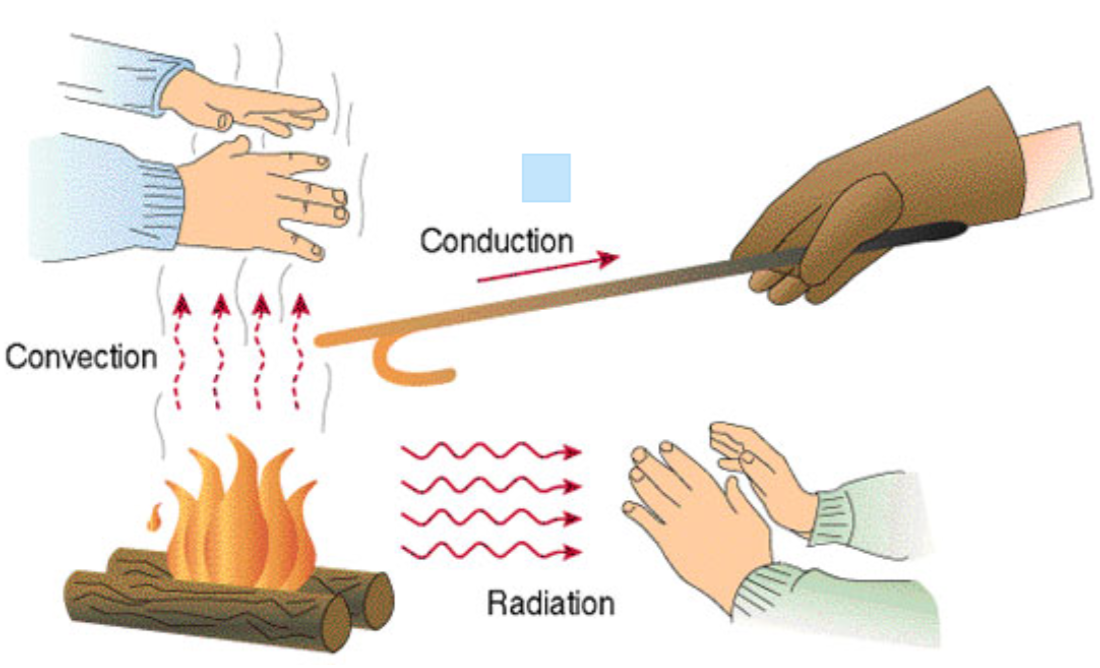
\includegraphics[scale=0.3]{ch1/1}
	\end{wrapfigure}
	Here is a picture illustrating the principles of \textbf{convection}, \textbf{conduction} and \textbf{radiation}. Imagine that you have a fire and you put your hands above. You will feel a flow of heat transmitted by convection. If someone comes with a stick, it will be conduction in the material transmitting the energy from particles to particles. Finally, if the hands are next to the fire, there is no flow but you feel the heat. The energy is transmitted by radiation. 
	
\subsection{Convection}
	\begin{wrapfigure}[4]{r}{4cm}
	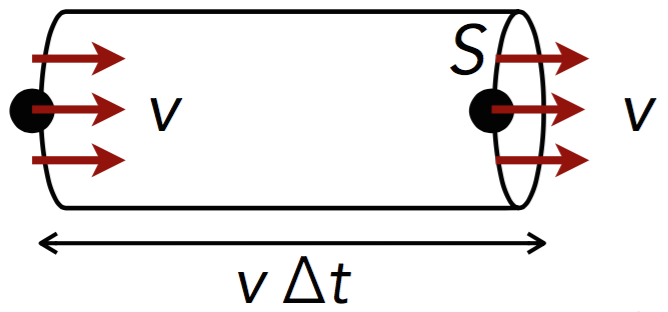
\includegraphics[scale=0.3]{ch1/2}
	\end{wrapfigure}
	Convection is a transfer always associated to bulk fluid motion. We consider a fluid with \textbf{uniform} velocity and a cylinder of section S and lenght $\Delta t$. In that time interval, the fluid in the cylinder will have crossed the section S. We are now able to express the convective flux of momentum, energy and mass knowing that the flux of a physical quantity is given by 
	\begin{equation}
	flux _A = \frac{A}{S\Delta t}
	\end{equation}
		
	
	

